\input{preamble.tex}

\title{High Cardinality Metrics}
\subtitle{I Am Not a Vendor}
\institute{DevOps Observability Architect}
\author{Jack Neely\\ jjneely@gmail.com}

\date{\today}

\usepackage[most]{tcolorbox}
\newtcolorbox{quotebox}{
    lower separated=false,
    arc=0pt,boxrule=0pt,leftrule=2pt
}

\begin{document}

\maketitle

\begin{frame}
    \frametitle{What are High Cardinality Metrics?}

    \begin{block}{metric: noun}
        A standard of measurement.\\
        \emph{``No metric exists that can be applied directly to happiness.''}
    \end{block}
    \begin{block}{cardinality: noun}
        The number of elements in a given mathematical set.\\
        \emph{``The set of real numbers has a bigger cardinality than the
        natural numbers because there are more of them.''}
    \end{block}

    \hspace*{\fill} -- Merriam Webster
\end{frame}

%% 'Curse of Dimenionality': Richard E. Bellman when considering problems in
%% dynamic programming.  1950s.
\begin{frame}[standout]
    \huge
    High Cardinality Metrics

    \Large
    The set of features being cataloged is greater than the set of data points
    or samples.
\end{frame}

%% TSDB Data Structure
\begin{frame}[plain]
\centering
\resizebox{!}{\textheight}{%
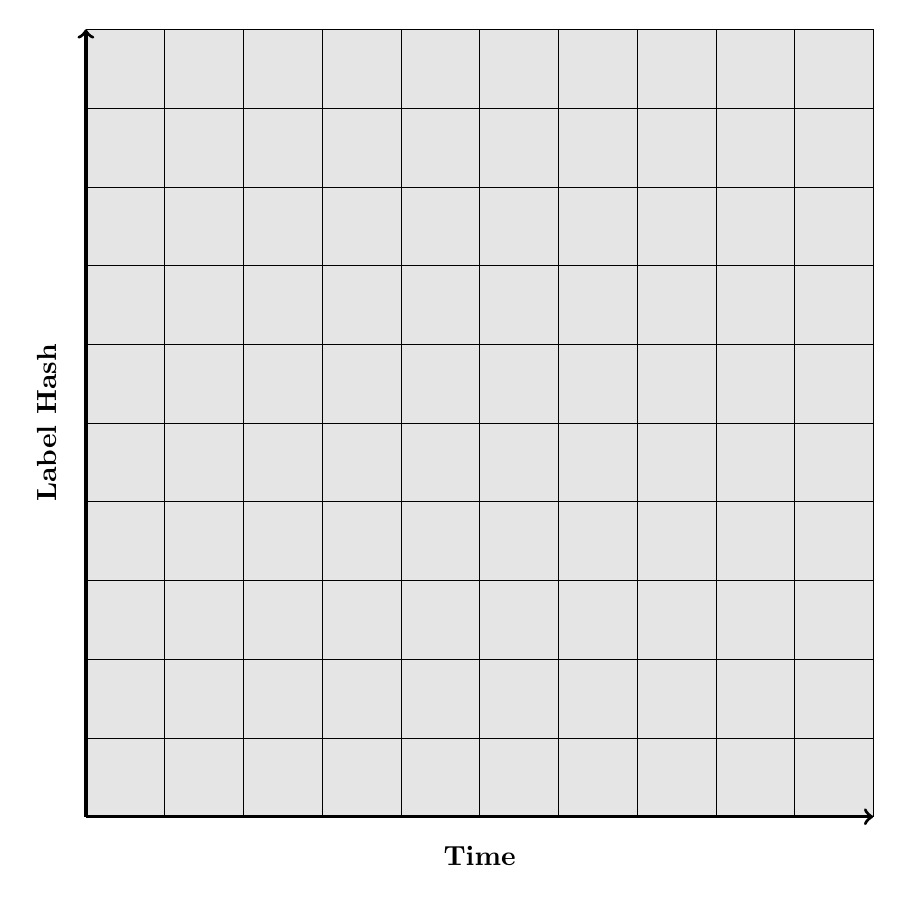
\begin{tikzpicture}
\fill [black!10!white] (0,0) rectangle (10,10);
\draw[step=1cm,black,very thin] (0,0) grid (10,10);
\draw[very thick,->] (0,0) -- (0,10);
\draw[very thick,->] (0,0) -- (10,0);
\draw (-0.5, 5) node[rotate=90] {\bf Label Hash};
\draw (5, -0.5) node {\bf Time};
\end{tikzpicture}}
\end{frame}

%% Well populated TSDB
\begin{frame}[plain]
\centering
\resizebox{!}{\textheight}{%
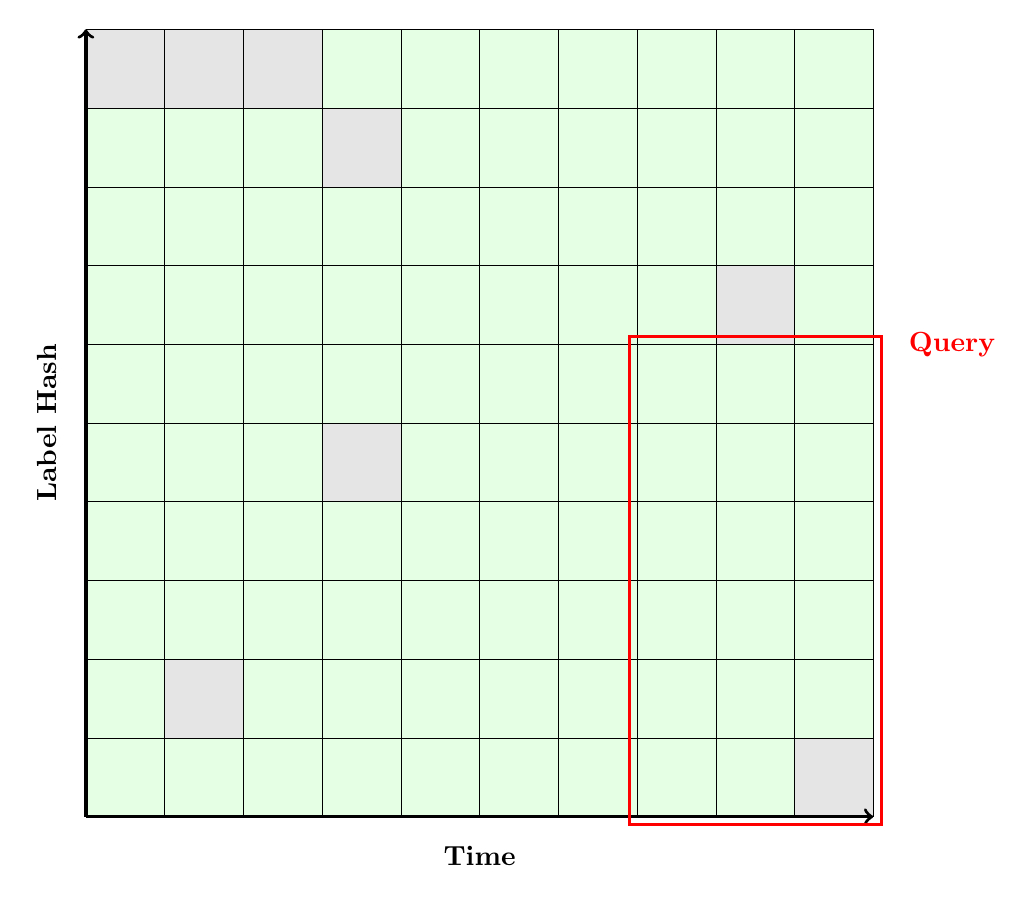
\begin{tikzpicture}
\fill [green!10!white] (0,0) rectangle (10,10);
\fill [black!10!white] (0,9) rectangle (3,10);
\fill [black!10!white] (1,1) rectangle (2,2);
\fill [black!10!white] (3,4) rectangle (4,5);
\fill [black!10!white] (3,8) rectangle (4,9);
\fill [black!10!white] (8,6) rectangle (9,7);
\fill [black!10!white] (9,0) rectangle (10,1);
\draw[step=1cm,black,very thin] (0,0) grid (10,10);
\draw[very thick,->] (0,0) -- (0,10);
\draw[very thick,->] (0,0) -- (10,0);
\draw (-0.5, 5) node[rotate=90] {\bf Label Hash};
\draw (5, -0.5) node {\bf Time};

\draw[red, very thick] (6.9, -0.1) rectangle (10.1, 6.1);
\draw [red] (11, 6) node {\bf Query};
\end{tikzpicture}}
\end{frame}

\begin{frame}
    \frametitle{Space Complexity (Big O Notation)}
    \Huge
    $$ O(n^2) $$
\end{frame}

\begin{frame}[plain]
\centering
\resizebox{!}{\textheight}{%
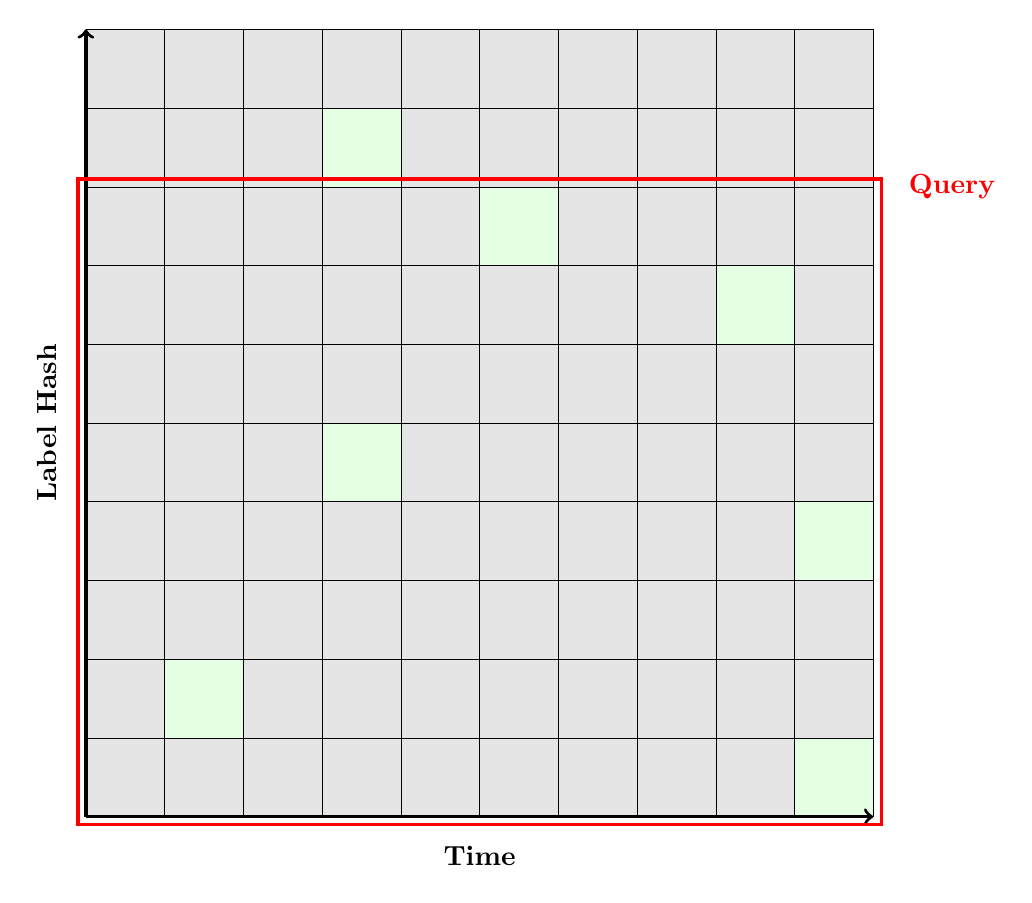
\begin{tikzpicture}
\fill [black!10!white] (0,0) rectangle (10,10);
\fill [green!10!white] (1,1) rectangle (2,2);
\fill [green!10!white] (3,4) rectangle (4,5);
\fill [green!10!white] (3,8) rectangle (4,9);
\fill [green!10!white] (8,6) rectangle (9,7);
\fill [green!10!white] (9,0) rectangle (10,1);
\fill [green!10!white] (5,7) rectangle (6,8);
\fill [green!10!white] (9,3) rectangle (10,4);
\draw[step=1cm,black,very thin] (0,0) grid (10,10);
\draw[very thick,->] (0,0) -- (0,10);
\draw[very thick,->] (0,0) -- (10,0);
\draw (-0.5, 5) node[rotate=90] {\bf Label Hash};
\draw (5, -0.5) node {\bf Time};

\draw[red, very thick] (-0.1, -0.1) rectangle (10.1, 8.1);
\draw [red] (11, 8) node {\bf Query};
\end{tikzpicture}}
\end{frame}

\begin{frame}[standout]

    More Metrics:  Shard

    Sparse Metrics:  Wrong solution
\end{frame}

\begin{frame}
    \frametitle{The Problem You Really Have}

    ``The Apache Problem''

    \begin{itemize}
        \item Are the data points aggregations?
        \item Is this data transactional?
        \item How important is this data, really?
        \item Does the data contain unique customer identifiers?
    \end{itemize}

\end{frame}

\end{document}
